\documentclass[svgnames]{amsart}
\usepackage[paperwidth=6in, paperheight=8in, top = 20mm, bottom = 18mm, left=10mm, right = 10mm]{geometry}

\usepackage{amsmath, amsfonts, amssymb, amsthm}
\usepackage{graphicx, tikz}
\usepackage{mathtools, physics}

\usepackage{enumitem}
\setlist[enumerate,1]{label=\arabic*.}

\usepackage[default,bold]{sourceserifpro}
\usepackage[T1]{fontenc}
\usepackage{eulervm}

\usepackage{xcolor}
\usepackage{scrlayer-scrpage}
\ohead{\color{blue!35!black} \scshape VM}
\cfoot*{\pagemark}

\renewcommand{\th}{\textsuperscript{th}}

\setlength{\parindent}{0pt}

\title[]{Probability and Statistics -- Problem Set 3}

\DeclareMathOperator{\Prob}{P}
\DeclareMathOperator{\EV}{\mathbb E}
\DeclareMathOperator{\Var}{\mathbb V}


\begin{document}
\maketitle
\begin{enumerate}[leftmargin=*]
\item $X \sim U[a,b]$, $a < 1 < 2 < b$. If $\Prob[X < 1] = 2\Prob[X > 2]$, and $5\Prob[X > 1] = 3\Prob[X < 2]$, find the values of $a$ and $b$.

\item $X$ is a discrete random variable taking values $0, 1, 2, \ldots$, whose pmf $f(x)$ is such that $\dfrac{f(x_1)}{f(x_2)} = r^{x_1 - x_2}$ for all $x_1, x_2 = 0, 1, 2, \ldots$ (where $r \in (0, 1)$ is a constant). Determine $f(x)$ and compute $\EV[X]$.

\item Let $X$ be the random variable with pdf $f(x)$ whose graph is shown below (where $a < b < c$ are three real numbers).\\
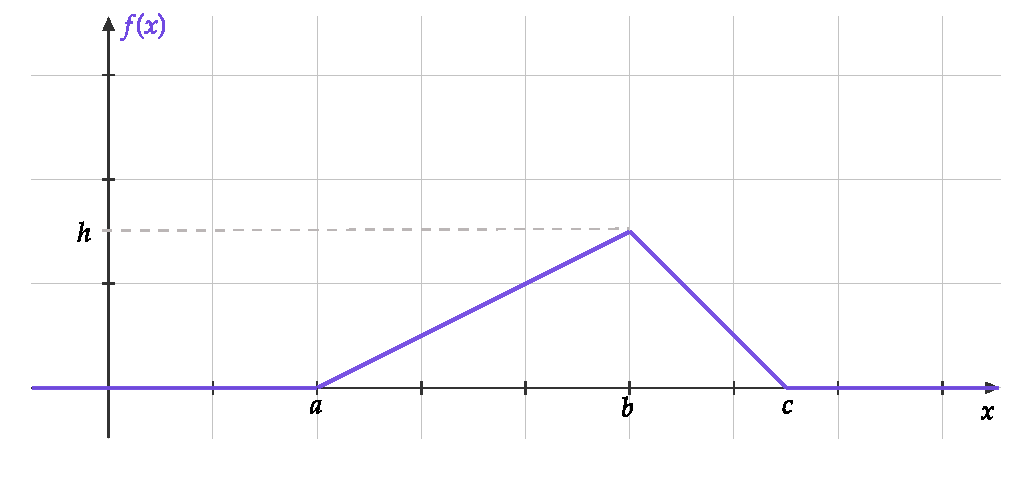
\includegraphics[scale=0.6]{Set3Graph.pdf}\\
Find $h$, and compute $\EV[X]$.

\item Show that the function
\begin{equation*}
f(x) = \dfrac{\lambda^x}{x!}e^{-\lambda}, x = 0, 1, 2, \ldots
\end{equation*}
(where $\lambda > 0$ is a constant) is a valid pmf, and compute $\EV[X]$ and $\Var[X]$.

\item $X$ is a discrete random variable with pmf $f(x) = \dfrac{6}{\pi^2 x^2}$, $x = 1, 2, \ldots$.
\begin{enumerate}
	\item Compute $\Prob[X \ge 3]$
	\item Compute $\Prob[10 \le X \le 15]$
	\item Show that $\EV[X]$ does not exist.
\end{enumerate}

\item $X$ is a continuous random variable with pdf $f(x) = \dfrac 6 {\pi^2} \pqty{\dfrac 1 {\lfloor x \rfloor}}^2$, $x > 1$.
\begin{enumerate}
	\item Compute $\Prob[X \ge 3]$
	\item Compute $\Prob[10 \le X \le 15]$
	\item Show that $\EV[X]$ does not exist.
\end{enumerate}

\item $X$ has pdf $f(x) = \dfrac{x^2}{3}$, $-1 \le x \le 2$. Compute
\begin{enumerate}
	\item $\Prob \bqty{X < \frac 3 2}$
	\item $\Prob[|X| > 1]$
	\item $\Prob \bqty{X < \frac 3 2 \mid X > \frac 1 2}$
	\item $\Prob \bqty{X < \frac 3 2 \mid |X| > 1}$
	\item $\Prob \bqty{|X| < 1 \mid X < \frac 3 2}$.
\end{enumerate}

\item An urn initially has {\color{red} $1$ red} and {\color{blue} $1$ blue} marble. A marble is drawn at random from the urn, and if it is {\color{blue} blue}, it is put back and {\color{red} one red} marble is added to the urn. This is continued until a {\color{red} red} marble is drawn. Let $X$ denote the total number of draws required to obtain a {\color{red} red} marble. Determine the probability distribution of $X$, and find its mean and variance.
{\scriptsize\textbf{Hint}: Compute $\EV[X + 1]$ and $\EV[X^2 - 1]$.}

\item The \emph{median} of a random variable $X$ is the point $c$ such that $\Prob[X \le c] = \Prob[X \ge c] = \frac 1 2$. Compute the median of $X$ with pdf $f(x)$ in each of the following cases.
\begin{enumerate}[itemsep=1em]
	\item $f(x) = \dfrac 1 {b - a}$, $a < x < b$.
	\item $f(x) = a e^{-ax}$, $x > 0$ [where $a > 0$ is a constant].
	\item $f(x) = \dfrac{1}{\pi(1 + x^2)}$ [Note that this distribution has no mean, but has a median].
\end{enumerate}
\end{enumerate}
\end{document}